\documentclass{article}

% Packages required to support encoding
\usepackage{ucs}
\usepackage[utf8x]{inputenc}
\usepackage{graphicx} 
% Packages required by code

% Packages always used
\usepackage{listings}
\usepackage{hyperref}
\usepackage{xspace}
\usepackage[usenames,dvipsnames]{color}
\hypersetup{colorlinks=true,urlcolor=blue}


\usepackage[framed,numbered,autolinebreaks,useliterate] {mcode}


\usepackage{geometry}
\geometry{letterpaper,textwidth=350pt,textheight=680pt,tmargin=60pt,
            left=72pt,footskip=24pt,headsep=18pt,headheight=14pt}
\usepackage{amsmath}
\usepackage{amssymb}
\usepackage{textcase}
\usepackage{soul}

\newcommand{\mat}[1]{\boldsymbol{#1}}\renewcommand{\vec}[1]{\boldsymbol{\mathrm{#1}}}
\newcommand{\vecalt}[1]{\boldsymbol{#1}}

\newcommand{\conj}[1]{\overline{#1}}

\newcommand{\normof}[1]{\|#1\|}
\newcommand{\onormof}[2]{\|#1\|_{#2}}

\newcommand{\itr}[2]{#1^{(#2)}}
\newcommand{\itn}[1]{^{(#1)}}

\newcommand{\eps}{\varepsilon}
\newcommand{\kron}{\otimes}

\DeclareMathOperator{\diag}{diag}
\DeclareMathOperator{\trace}{trace}
\DeclareMathOperator{\tvec}{vec}

\newcommand{\prob}{\mathbb{P}}
\newcommand{\probof}[1]{\prob\left\{ #1 \right\}}

\newcommand{\pmat}[1]{\begin{pmatrix} #1 \end{pmatrix}}
\newcommand{\bmat}[1]{\begin{bmatrix} #1 \end{bmatrix}}
\newcommand{\spmat}[1]{\left(\begin{smallmatrix} #1 \end{smallmatrix}\right)}
\newcommand{\sbmat}[1]{\left[\begin{smallmatrix} #1 \end{smallmatrix}\right]}

\newcommand{\RR}{\mathbb{R}}
\newcommand{\CC}{\mathbb{C}}

\providecommand{\eye}{\mat{I}}
\providecommand{\mA}{\ensuremath{\mat{A}}}
\providecommand{\mB}{\ensuremath{\mat{B}}}
\providecommand{\mC}{\ensuremath{\mat{C}}}
\providecommand{\mD}{\ensuremath{\mat{D}}}
\providecommand{\mE}{\ensuremath{\mat{E}}}
\providecommand{\mF}{\ensuremath{\mat{F}}}
\providecommand{\mG}{\ensuremath{\mat{G}}}
\providecommand{\mH}{\ensuremath{\mat{H}}}
\providecommand{\mI}{\ensuremath{\mat{I}}}
\providecommand{\mJ}{\ensuremath{\mat{J}}}
\providecommand{\mK}{\ensuremath{\mat{K}}}
\providecommand{\mL}{\ensuremath{\mat{L}}}
\providecommand{\mM}{\ensuremath{\mat{M}}}
\providecommand{\mN}{\ensuremath{\mat{N}}}
\providecommand{\mO}{\ensuremath{\mat{O}}}
\providecommand{\mP}{\ensuremath{\mat{P}}}
\providecommand{\mQ}{\ensuremath{\mat{Q}}}
\providecommand{\mR}{\ensuremath{\mat{R}}}
\providecommand{\mS}{\ensuremath{\mat{S}}}
\providecommand{\mT}{\ensuremath{\mat{T}}}
\providecommand{\mU}{\ensuremath{\mat{U}}}
\providecommand{\mV}{\ensuremath{\mat{V}}}
\providecommand{\mW}{\ensuremath{\mat{W}}}
\providecommand{\mX}{\ensuremath{\mat{X}}}
\providecommand{\mY}{\ensuremath{\mat{Y}}}
\providecommand{\mZ}{\ensuremath{\mat{Z}}}
\providecommand{\mLambda}{\ensuremath{\mat{\Lambda}}}
\providecommand{\mPbar}{\bar{\mP}}

\providecommand{\ones}{\vec{e}}
\providecommand{\va}{\ensuremath{\vec{a}}}
\providecommand{\vb}{\ensuremath{\vec{b}}}
\providecommand{\vc}{\ensuremath{\vec{c}}}
\providecommand{\vd}{\ensuremath{\vec{d}}}
\providecommand{\ve}{\ensuremath{\vec{e}}}
\providecommand{\vf}{\ensuremath{\vec{f}}}
\providecommand{\vg}{\ensuremath{\vec{g}}}
\providecommand{\vh}{\ensuremath{\vec{h}}}
\providecommand{\vi}{\ensuremath{\vec{i}}}
\providecommand{\vj}{\ensuremath{\vec{j}}}
\providecommand{\vk}{\ensuremath{\vec{k}}}
\providecommand{\vl}{\ensuremath{\vec{l}}}
\providecommand{\vm}{\ensuremath{\vec{l}}}
\providecommand{\vn}{\ensuremath{\vec{n}}}
\providecommand{\vo}{\ensuremath{\vec{o}}}
\providecommand{\vp}{\ensuremath{\vec{p}}}
\providecommand{\vq}{\ensuremath{\vec{q}}}
\providecommand{\vr}{\ensuremath{\vec{r}}}
\providecommand{\vs}{\ensuremath{\vec{s}}}
\providecommand{\vt}{\ensuremath{\vec{t}}}
\providecommand{\vu}{\ensuremath{\vec{u}}}
\providecommand{\vv}{\ensuremath{\vec{v}}}
\providecommand{\vw}{\ensuremath{\vec{w}}}
\providecommand{\vx}{\ensuremath{\vec{x}}}
\providecommand{\vy}{\ensuremath{\vec{y}}}
\providecommand{\vz}{\ensuremath{\vec{z}}}
\providecommand{\vpi}{\ensuremath{\vecalt{\pi}}}

\sodef\allcapsspacing{\upshape}{0.15em}{0.65em}{0.6em}%

\makeatletter
\def\maketitle{%
\par
\hrule height 0.75pt\vspace{1ex}
\par\noindent
\begin{minipage}{0.5\textwidth}
\scshape
purdue university $\cdot$ CS 580 \\
Introduction to the Analysis of Algorithms
\end{minipage}
\begin{minipage}{0.5\textwidth}
\raggedleft
\MakeTextUppercase{\allcapsspacing{\@title}}\\[0.2ex]
\textit{\@author}\\[0.2ex]
\textit{\@date}
\end{minipage}
\par\vspace{1ex}
\hrule height 1pt
\vspace{2ex}
\par
}
\makeatother

\author{Jun Cheng}
\title{Lecture Notes}
% auto generate a title
\AtBeginDocument{\maketitle}


\title{Homework}



\begin{document} 



\hypertarget{problem_0_homework_checklist_2}{}
\subsection*{{Problem 0: Homework checklist}}
\label{}

\checkmark	I didn't talk with any one about this homework. \newline
\checkmark 	Source-code are included at the end of this document. 

\hypertarget{}{}
\subsection*{{Problem 1: GERSHGORIN DISKS }}

\begin{enumerate} 
\item 
Suppose $\mA$ is a complex $n\times n$ matrix, with $a_{ij}$. Compute all the sum of the absolute values of the non-diagnonal entries in the i-th row $R_i=\sum_{j\neq i}|a_{ij}| $.   Then if we draw some closed disc centered at $a_{ii}$ with radius $R_i$, each eigenvalue of $\mA$ lies in at least one of those discs.  Those discs are called Gershgorin disc.  
\item 
The function for ploting Gershgorin Discs is shown as below: \\
\begin{lstlisting} 
function h= plotDisk(A); 
[n,m] = size(A); 
R =zeros(n, 1); 
lam = eig(A); 
for i=1:n 
    for j=1:n
        if i~=j
            R(i)=R(i)+abs(A(i,j)); 
        end
    end
    %diskPlot(A(i,i), 0, R(i)); 
    th = 0:pi/50:2*pi;
    xunit = R(i) * cos(th) + A(i,i);
    yunit = R(i) * sin(th) + 0;
    h = plot(xunit, yunit);
    scatter(lam(i), 0, 100); 
    axis equal; 
    hold on; 
end
end
\end{lstlisting} 

\item
The Gershgorin discs plot is shown in Figure 1. \\
\begin{figure}
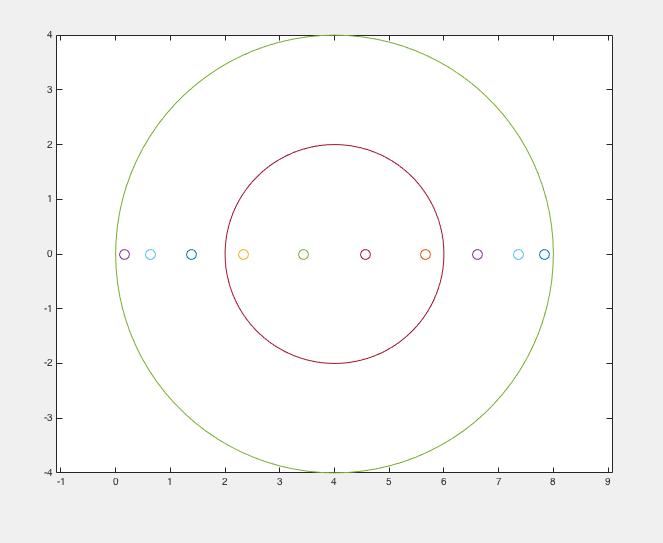
\includegraphics[width=0.7\textwidth]{problem1_3} 
\centering 
\caption{The Gershgorin discs for a matrix in Problme 1.3. All the small circle are the position of true eigenvalues.} 
\end{figure}
\end{enumerate}

\hypertarget{}{}
\subsection*{{Problem 2:More eigenvalues and convergence theory}}
\label{}

\begin{enumerate} 
\item 
To show that the Jacobi iteration converges for 2-by-2 symmetric, positive, definite systems,  the matrix $\mA$ 
satisfies $\vx^T\mA\vx >0 (\forall x\neq0) $ 
\begin{align*} 
\mA &=\bmat{a & c \\ c& b} \\
\mA &= \mD +\mR \\
\mD &= \bmat{a & 0 \\ 0 & b} \\
\mR & = \bmat{0 & c \\ c & 0 } \\
\end{align*} 
Then the Jacobian iteration is $ \vx^{(k+1)} = \mD^{-1} (\vb-\mR\vx^{(k))}$. \\ 
For a symmetric definite matrix, we have $a>0, b>0$ and $det(\mA)>0$. \\
\begin{align*}
det(\mA) = ab-c^2 >0 \\
\frac{c^2}{ab}<1 \\
\end{align*}
Then  \begin{align*} 
det(\mD^{-1}\mR-\lambda \mI) = \lambda^2-\frac{c^2}{ab} \\
|\lambda|<1 
\end{align*} 
Then we know that the absolute value of all eigenvalues for $\mD^{-1}\mR$ are smaller than 1. \\
\begin{align*} 
\rho(\mD^{-1}\mR)<1\\
\end{align*}
That indicates the Jacobian iteration method converges. \\

\item 
If $\rho(\mM^{-1}\mN)<1$  and $e^{(k)} = e^{(k)} -x$ 
\begin{align*} 
e^{(k)} &=\mM^{-1}\mN e^{(k-1)} \\
& = \mG e^{(k-1)} \\
& = \mG^ke^{(0)} \\
\mM(\vx^{(k)}-x)  &= \mN(x^{(k-1)}-x)
\end{align*} 
This is the solution of equation $\mM\vx = \mN\vx = \vb $ and $\mA\vx = \vb$ where $\mA=\mM+\mN$.  
Then the matrix $\mA$ can not be a singular matrix. Therefore if $\mA$ is singular, then we can never have $\rho(\mM^{-1}\mN)<1$. \\
 


\end{enumerate} 




\end{document}
